Detta arbete presenterar AMBA (\emph{Automatic manual binary analysis}), ett
binäranalysverktyg för att visualisera och styra symbolisk fuzzing interaktivt.
I detta avsnitt kommer vi att beskriva funktionalitet i AMBA, AMBAs
begräsningar samt hur man kan köra och använda AMBA.

AMBA exekverar program med symbolisk indata och visar ett antal grafer
över exekveringen. Dessa grafer uppdateras kontinuerligt under programmets
exekvering. Graferna består av ett antal noder med metadata sammankopplade
med riktade kanter. När en användare klickar på en nod visas den nodens metadata
i en separat panel. Metadatan visas även om man zoomar in på en nod.

\begin{figure}
    \centering
    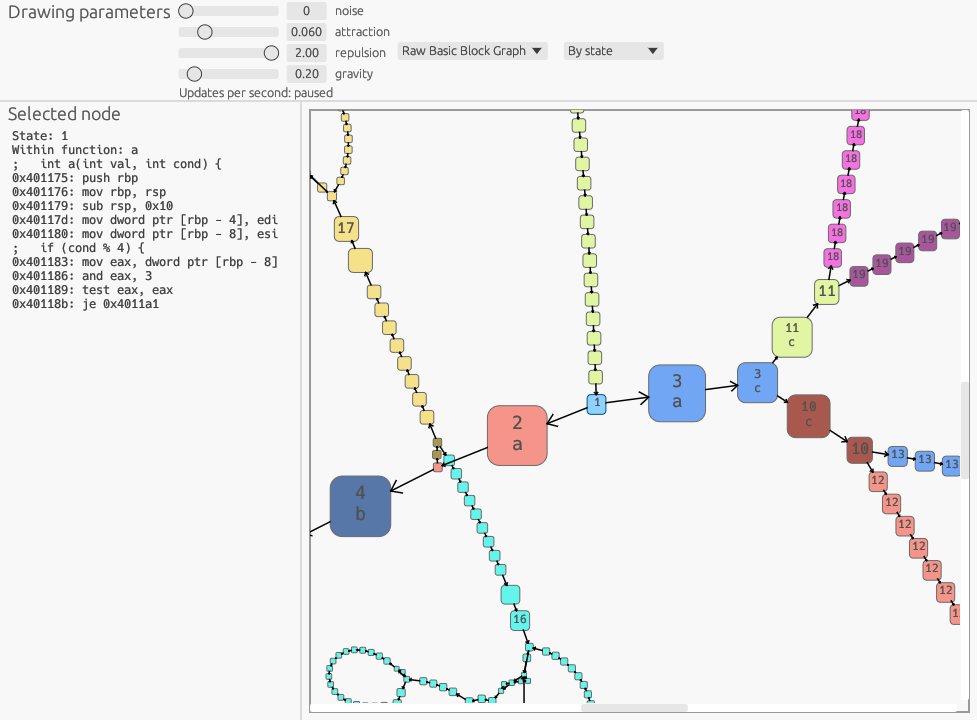
\includegraphics[width=0.7\textwidth]{figures/graph_basic_block.png}
    \caption{
        AMBAs basic-block-graf för testprogrammet control-flow
    }\label{fig:graf-basic}
\end{figure}

Den första grafen är en basic-block-graf. Figur~\ref{fig:graf-basic} visar ett
exempel. Här representerar varje tillstånd i grafen ett basic block i
maskinkoden, alltså en sekvens maskinkod som exekveras utan hopp. Det grafiska
gränssnittet visar blockets adress, det symboliska tillståndet blocket exekveras
i och den disassemblerade maskinkoden. Om binären innehåller debugdata visas
även funktionsnamn och om både debugdata och källkoden är tillgänglig visas de
källkodsrader som gett upphov till maskinkoden.

\begin{figure}
    \centering
    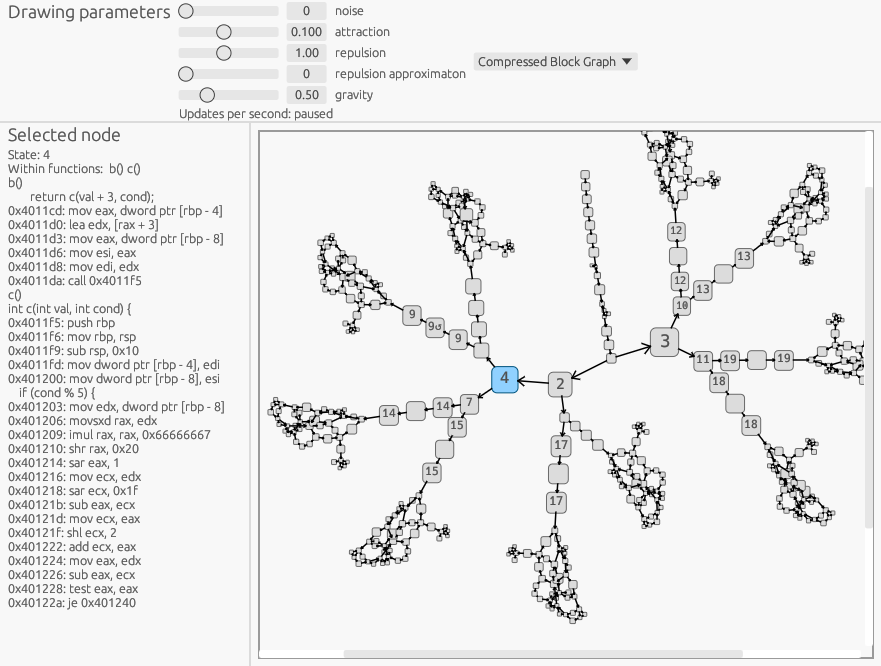
\includegraphics[width=0.7\textwidth]{figures/graph_block_compressed.png}
    \caption{
        AMBAs komprimerade basic-block-graf för testprogrammet control-flow
    }\label{fig:graf-compressed}
\end{figure}

Den andra grafen är en komprimerad basic-block-graf.
Figur~\ref{fig:graf-compressed} visar ett exempel. Den visar samma graf som den
första, men med linjesubgrafer sammanslagna till samma nod. Precist uttryckt kantkomprimeras
alla kanter till noder som har ingrad och utgrad exakt ett. Sidopanelen visar samma information som för
basic-block-grafen, alltså assemblerkod och debugdata, men för hela spannet av
sammanslagna noder.

\begin{figure}
    \centering
    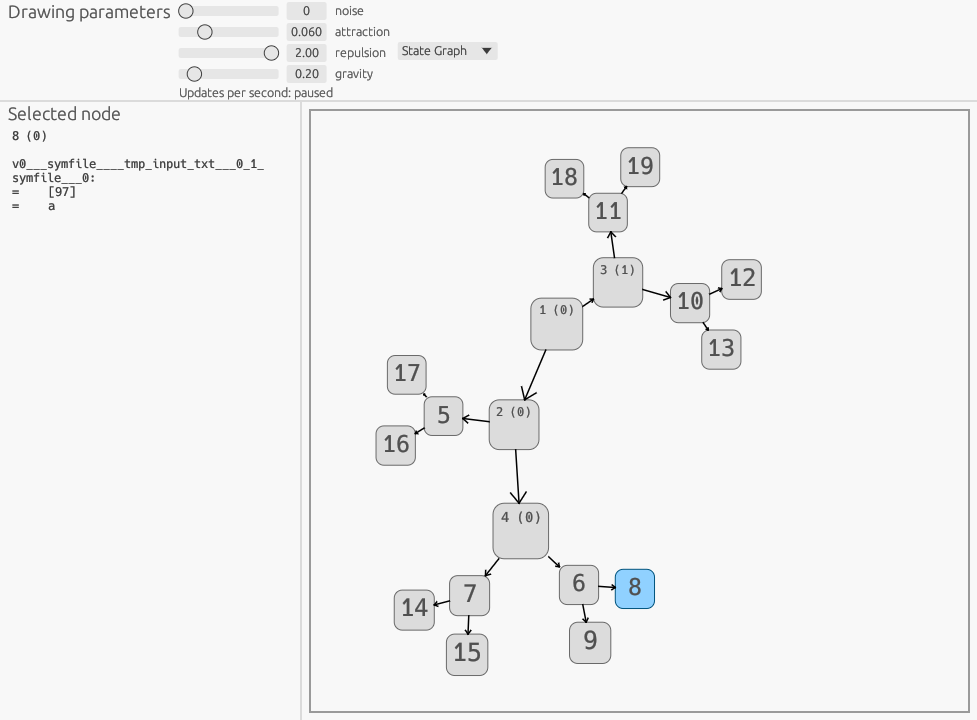
\includegraphics[width=0.7\textwidth]{figures/graph_symbolic.png}
    \caption{
        AMBAs graf över symboliska tillstånd för testprogrammet control-flow
    }\label{fig:graf-symbolic}
\end{figure}

Den tredje grafen visar symboliska tillstånd. Figur~\ref{fig:graf-symbolic}
visar ett exempel. Ett tillstånd utgörs av exekveringsspannet uppdelat vid varje
gren som görs baserat på ett symboliskt uttryck. Sidopanelen visar
tillståndets namn samt det grennummer som identiferar det föränderliga
tillståndet i \stoe{}. Då föräldrar inte kan samexistera i tid med sina barn
använder \stoe{} grennummer för att hänvisa till nu körande tillstånd.

\begin{figure}
    \centering
    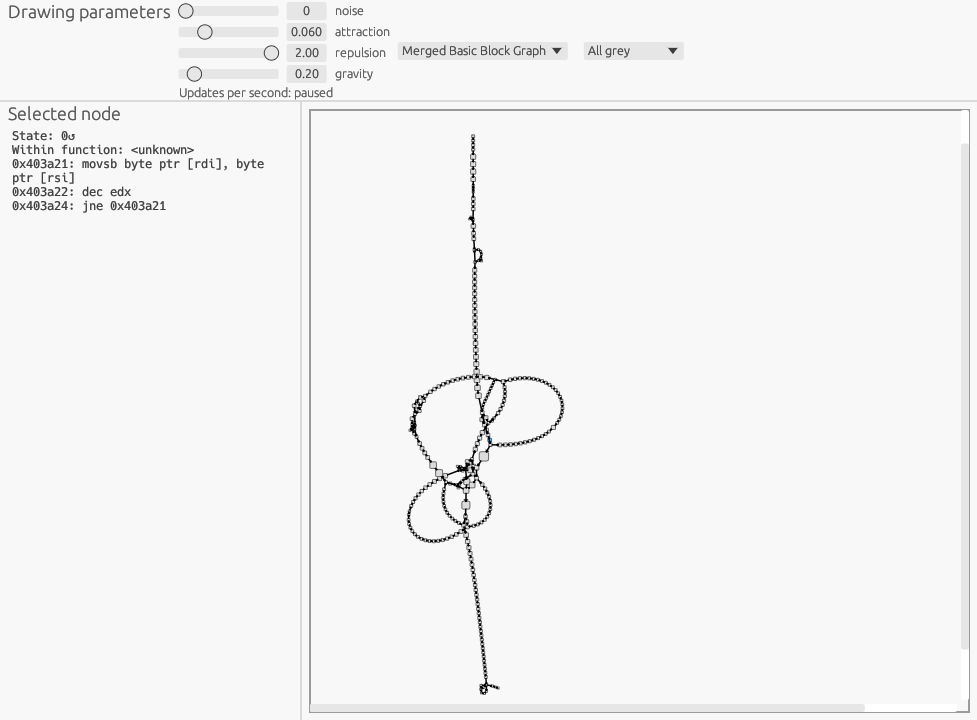
\includegraphics[width=0.7\textwidth]{figures/graph_merged.png}
    \caption{
        AMBAs sammanslagna basic-block-graf för testprogrammet control-flow
    }\label{fig:graf-merged}
\end{figure}

Den fjärde grafen är en sammanslagen basic-block-graf, som visar basic-block
utan att delas vid tillståndsdelning. Precist uttryckt är det grafen som bildas
från den första grafen, efter att varje par av noder vars metadata endast
skiljer sig i det symboliska tillståndet har ersatts med en nod kopplad till unionen av
de ursprungliga nodernas kanter. Figur~\ref{fig:graf-merged} visar ett exempel.

\begin{figure}
    \centering
    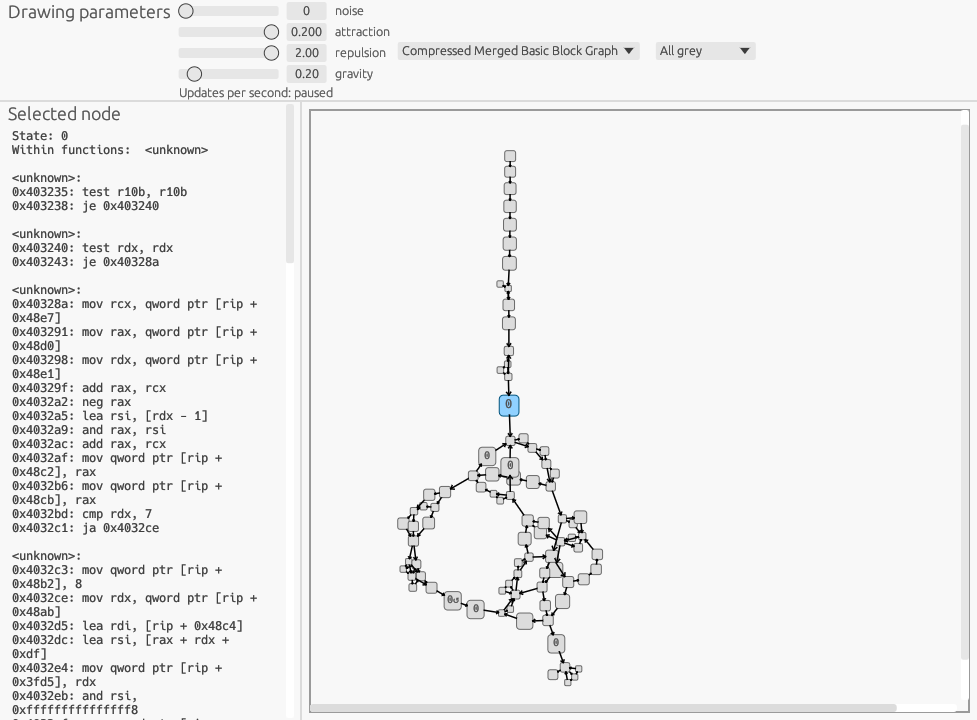
\includegraphics[width=0.7\textwidth]{figures/graph_merged_compressed.png}
    \caption{
        AMBAs komprimerade sammanslagna basic-block-graf för testprogrammet control-flow
    }\label{fig:graf-merged-compressed}
\end{figure}

Den femte och sista grafen är en komprimerad sammanslagen basic-block-graf,
vilken konstrueras från den sammanslagna basic-block-grafen genom samma
kompression som i den komprimerade block-block-grafen.
Figur~\ref{fig:graf-merged-compressed} visar ett exempel.

De två första graferna, alltså de komprimerade och okomprimerade
basic-block-graferna, kan färgläggas utifrån symboliska tillstånd och starkt
anslutna komponenter.

Utöver att visa dessa grafer går det också att välja noder i den symboliska
tillståndsgrafen för att prioritera deras fortsatta evaulering. Detta gör det
möjligt att undersöka intressanta subträd i grafer som är större än vad AMBA
realistiskt sett kan besöka och visa. Detta kan användas för att kringgå
vägexplosionsproblemet och undvika att enorma grafer skapas av program som inte
terminerar. Genom att dubbelklicka på en nod i tillståndsgrafen kommer
exekveringen fortsätta från motsvarande tillstånd.

Grafnodernas placering i 2D hittas genom iterativ lösning för lägst energi i ett
system av attraktion, repulsion och externa krafter. Utplaceringsalgoritmens
parametrar kan konfigureras i realtid vid körning av användaren i toppanelen.
Den här panelen låter även användaren välja vilken graf de vill visa.

Genom \stoe{} kör AMBA det analyserade programmet virtualiserat med KVM i
QEMU.\@ Detta innebär att den analyserade binärens beteende i hög grad inte
påverkas av miljön på datorn som kör AMBA, vilket gör analysen mer
reproducibel. Det innebär också att skadlig kod borde kunna analyseras dynamiskt
i AMBA med låg risk för skadlig påverkan på användarens dator. Dock är AMBA
omogen programvara som ej granskats för felkonfiguration eller liknande kopplat
till QEMU eller \stoe{}, så vi rekommenderar inte att använda AMBA för analys av
skadlig kod i dess nuvarande skick.

\section{Begränsningar}

Alla program kan inte hanteras av AMBA.\@ Programmen som AMBA kör måste vara
byggda för Linux x86-64 och kunna köras på Ubuntu-22.04-x86\_64. Detta kan göras
genom att bygga direkt för Ubuntu eller med full statisk länkning mot t.ex.\
libc-implementationen musl istället för dynamisk länkning mot glibc.

Den symboliska indatan är också begränsad till att komma ifrån stdin samt filer
på disk. Symbolisk input till AMBA i dess nuvarande skick kan inte skickas som
programargument (\verb|argc|, \verb|argv|), miljövariabler (\verb|envp|) eller i
form av symbolisk hårdvara (t.ex.\ registret TSC/Time Stamp Counter). Detta är
inte en fundamental begränsning utan endast oimplementerad funktionalitet som
lämnas som utvecklingsmöjlighet.

En stor begränsning vid användandet av AMBA och symbolisk fuzzing i
allmänhet är hanterandet av program med väldigt många symboliska tillstånd.
Detta problem kallas vägexplosionsproblemet och beskrivs i inledningen,
Sektion~\ref{chap:inledning}. AMBAs enda funktionalitet för att hantera detta är
prioritering av exekveringstillstånd, vilket är ett trubbigt verktyg. Detta är
till stor del en fundamental begränsning i symbolisk fuzzing och kräver
yttligare metoder för att försöka angripa problemet.

\section{Hur du kör AMBA}\label{sec:run-amba}

AMBA utvecklades i GitHub-repot
\url{https://github.com/lokegustafsson/amba-bsc-thesis}. Dokumentationen i repot
innehåller mer detaljerade installationsinstruktioner och allmän dokumentation.

AMBA kan köras i alla Linux-x86-64-miljöer med stöd för KVM med tillräckligt
mycket diskutrymme (ca $\SI{20}{\giga\byte}$) och RAM-minne
($\SI{16}{\giga\byte}$ för att bygga AMBA, ej nödvändigt vid nedladdning av
cachad binär). De tre installationsstegen består av att först installera
pakethanteraren Nix, följt utav av att köra kommandot \lstinline{nix build}.  När
detta kommandot körs byggs alla programvarukomponenter från LLVM och Linux till
\stoe{} och AMBA självt. Detta bygget är deterministiskt reproducibelt från
källkod och Nix möjliggör även korrekt cachelagring och servering över nätverk
vilket vi använt för att minimiera ombyggnation under AMBAs utvecklingsprocess.
Det sista installationssteget är att köra kommandot
\lstinline{nix run . -- init --download}
som laddar ned en Ubuntu-22.04-x86\_64-diskavbild byggd av \stoe{}-projektet
. Bygget av diskavbilder för \stoe{} är inte bit-för-bit reproducibelt
och därför är detta bygget inte packeterat i Nix.

AMBA körs med kommandot
\begin{verbatim}
./result/bin/amba-wrapped run path/to/a/recipe.json"
\end{verbatim}
efter \lstinline{nix build} eller ekvivalent
\begin{verbatim}
nix run . -- run path/to/a/recipe.json"
\end{verbatim}
alltså genom att peka AMBA på en receptfil. En giltig receptfil följer ett
schema varav en delmängd av fälten har implementerad funktionalitet.
Figur~\ref{fig:recipe} visar en receptfil för vilken alla fält är
implementerade.

\begin{figure}
    \begin{lstlisting}[
    language=json,
    frame=single
    ]
{
  "files": {
    "control-flow": "./control-flow",
    "input.txt": {
      "seed": "a",
      "symbolic": [0]
    }
  },
  "executable_path": "./control-flow",
  "stdin_path": "/tmp/input.txt"
}
\end{lstlisting}

    \caption{
        Receptfilen för testprogrammet control-flow. Binären
        \texttt{control-flow} ligger bredvid receptfilen och kopieras till
        QEMU-gästens hemmapp. Dessutom placeras en 1 byte lång fil innehållande en
        symbolisk variabel i \texttt{/tmp/input.txt}. I gästen körs binären med den
        symboliska filen som \texttt{stdin}.
    }\label{fig:recipe}

\end{figure}

I receptfilen specifieras först ett antal filer som ska placeras i QEMU-gästen.
Filerna specifieras med deras relativa sökväg i gästen, med konkreta filer
angivna relativt \verb|~/| och symboliska filer angivna relativt \verb|/tmp/|.
Filers innehåll kan specifieras som en sökväg relativt mappen receptfilen ligger
i, vilket kopierar in en konkret fil. Filers innehåll kan också specifieras som
symboliska genom att ange en lista av byteadresser (t.ex.\ \verb|0|) samt
byteadressintervall (t.ex.\ \verb|[42, 57]|) mellan vilka filen ska innehålla
symboliska bytes. Symboliska filer behöver också konkreta värden som får förtur
i tillståndsutforskningen. Dessa kan anges med antingen
\verb|"seed": "<förtursvärden>"| eller
\verb|"host_path": "<värddatorsökväg till förtursvärden>"|.

När AMBA körs med \lstinline{nix run . -- run path/to/a/recipe.json} öppnas det
grafiska gränssnittet samtidigt som QEMU/\stoe{} startas i bakgrunden.
Grafuppdateringar skickas regelbundet tillbaka tills alla tillstånd utforskats
eller programmet stänger ned. Både före och efter alla tillstånd utforskats kan
graferna undersökas av användaren.
